\chapter{Experimental results}
This chapter presents the results obtained from the design, starting from functional verification of the correctness of the implementation, to synthesis and benchmarking. The entire design has been described in SystemVerilog using hierarchical modules and behavioral constructs when possible. This both helps readability and leaves to the EDA tools the freedom of performing optimizations.

Each module has been verified locally using Verilator\footnote{\url{https://www.veripool.org/wiki/verilator}} for linting and Mentor ModelSim Intel \acs{FPGA} Starter Edition for simulation. Synthesis has been carried out with Synopsys Design Compiler, on the the VLSI server provided by Politecnico di Torino.

\section{Simulation}
The choice of tools mentioned above was made because one of the pros of Verilator is that it has been found to be more verbose than ModelSim when performing syntax check and lint, thus reducing the number of possible issues during compilation and simulation. Moreover, it is completely free and open source, which nicely couples with the philosophy of the LEN5 project.

ModelSim was in the end chosen as the main simulation tool, because it is much more familiar to the designer and the limited time did not allow to learn Verilator for simulation, given that it uses a completely different paradigm, based on translating \acs{HDL} to C language and using testbench templates in C as well.

The following sections focus on the test strategies used for the \ac{BPU}, which is almost as important as a standalone design, and the top-level frontend.

\subsection{\acs{BPU}}
The testbench of the \ac{BPU} is based on reading branch addresses from one file, predicting the outcome and then comparing it with the correct branch resolutions coming from a second file. One clock cycle passes between the prediction and the resolution, as to simulate the execution delay, which always takes more cycles. During this time span, the \ac{PC} is fictionally increased to simulate a normal sequential fetch situation.

Given that the length of the history register in the gshare and the length of \ac{BTB} address lead to an exponential growth of the \ac{PHT} and the \ac{BTB} itself, simulations were performed using a small number of bits for these data structures and in particular the following results refer to a configuration with a 4-bit history register and a 4-bit \ac{BTB} address. The simulation is needed to verify the correctness of the design and not the prediction performances, so having fewer bits poses no issues.

In order to test the \ac{BPU} as a singular unit, without all the surrounding processor and in particular without a register file and execution units, some specific test cases have been defined, where branch results could be derived manually without actually executing the program. Loops, in particular, suit well such simple cases.

\subsubsection{Single loop}
The first test case corresponds to the following simple loop:
\begin{lstlisting}[language=C]
  for (int i = 0; i < 10; i++)
  {
    /* loop body */
  }
\end{lstlisting}
Here, the loop condition is tested ten times as true, so the branch is taken, and the last time as false, so the branch is not taken.

\begin{sidewaysfigure}[p]
  \centering
  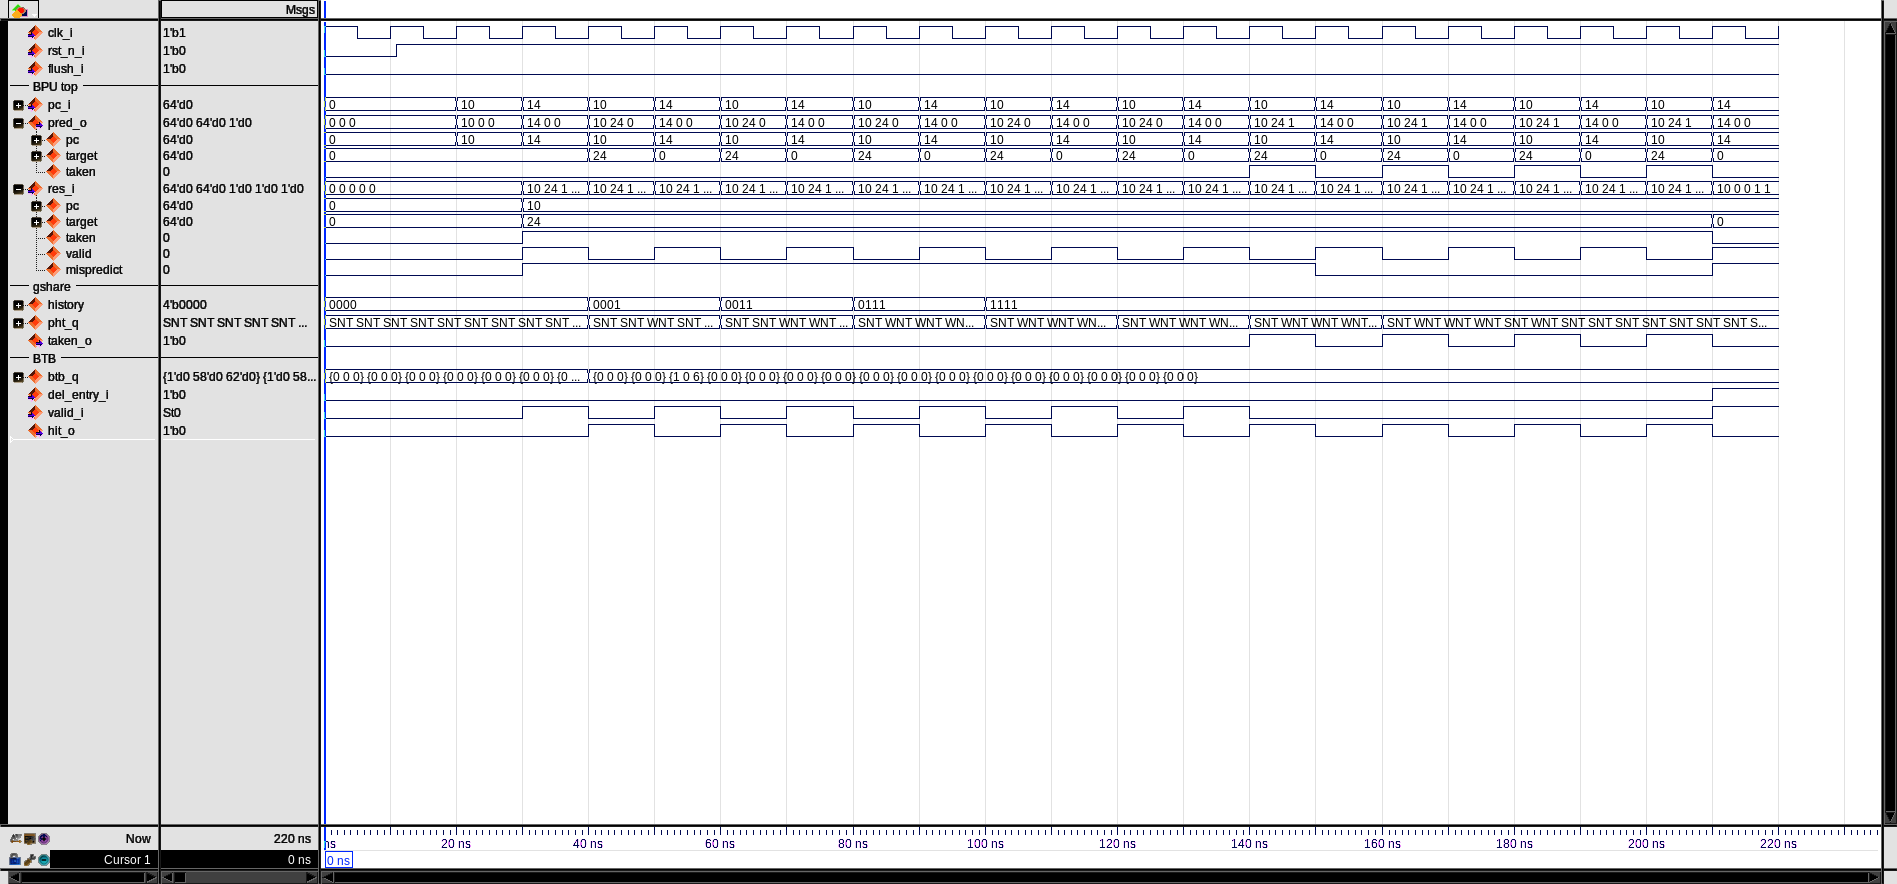
\includegraphics[width=\textheight]{img/bpu_loop01_conv.png}
  \caption{Single loop simulation}
  \label{fig:bpu_loop01_conv}
\end{sidewaysfigure}
Suppose that the instruction testing the loop condition is at address 10 and the beginning of the loop body (i.e. the target of the branch instruction) is at address 24. \Cref{fig:bpu_loop01_conv} shows the simulation waveforms for this test case, with the predictions contained in the \texttt{pred\_o} signal, occurring each time the \ac{PC} 10 is read from the address file, and the resolutions read into \texttt{res\_i} every time the \texttt{valid} signal is asserted.

Here, the initialization of the predictor structures can be clearly noted. Given that the history register is initialized to zero and the loop branch is always taken at first, the gshare predictor will initially update 2-bit counters which do not correspond to the actual branch history, until the \ac{BHT} is filled with ones (4 iterations, for the 4-bit register). Then the \ac{PHT} index will remain the same and so the same 2-bit counter is incremented from the initial strongly not taken state to the weakly taken state when it finally starts predicting correctly (2 iterations).

At the seventh iteration of the loop, the branch is predicted correctly as taken (the \texttt{mispredict} signal is deasserted) and this situation lasts until the the loop condition is tested false at the last iteration, leading to a new misprediction. 

Meanwhile, the \ac{BTB} is updated with the correct target at the first iteration, from which it gets a hit each following time.

This \emph{warm-up} of the predictor is intrinsic of its design and cannot be avoided, but anyway \cref{fig:bpu_loop01_conv} demonstrates the correct and expected behavior of the \ac{BPU}.

\subsubsection{Nested loops}
Next, the case of two nested loops was tested, as in the following code:
\begin{lstlisting}[language=C]
  for (int i = 0; i < 20; i++)
  {
    for (int j = 0; j < 3; j++)
    {
      /* loop body */
    }
  }
\end{lstlisting}
This example, actually taken from \cite{mcfarling93}, is intended to demonstrate that the gshare predictor, after the warm-up, can correctly identify taken branches in nested loops, where the outer loop is repeated many times.

\begin{sidewaysfigure}[p]
  \centering
  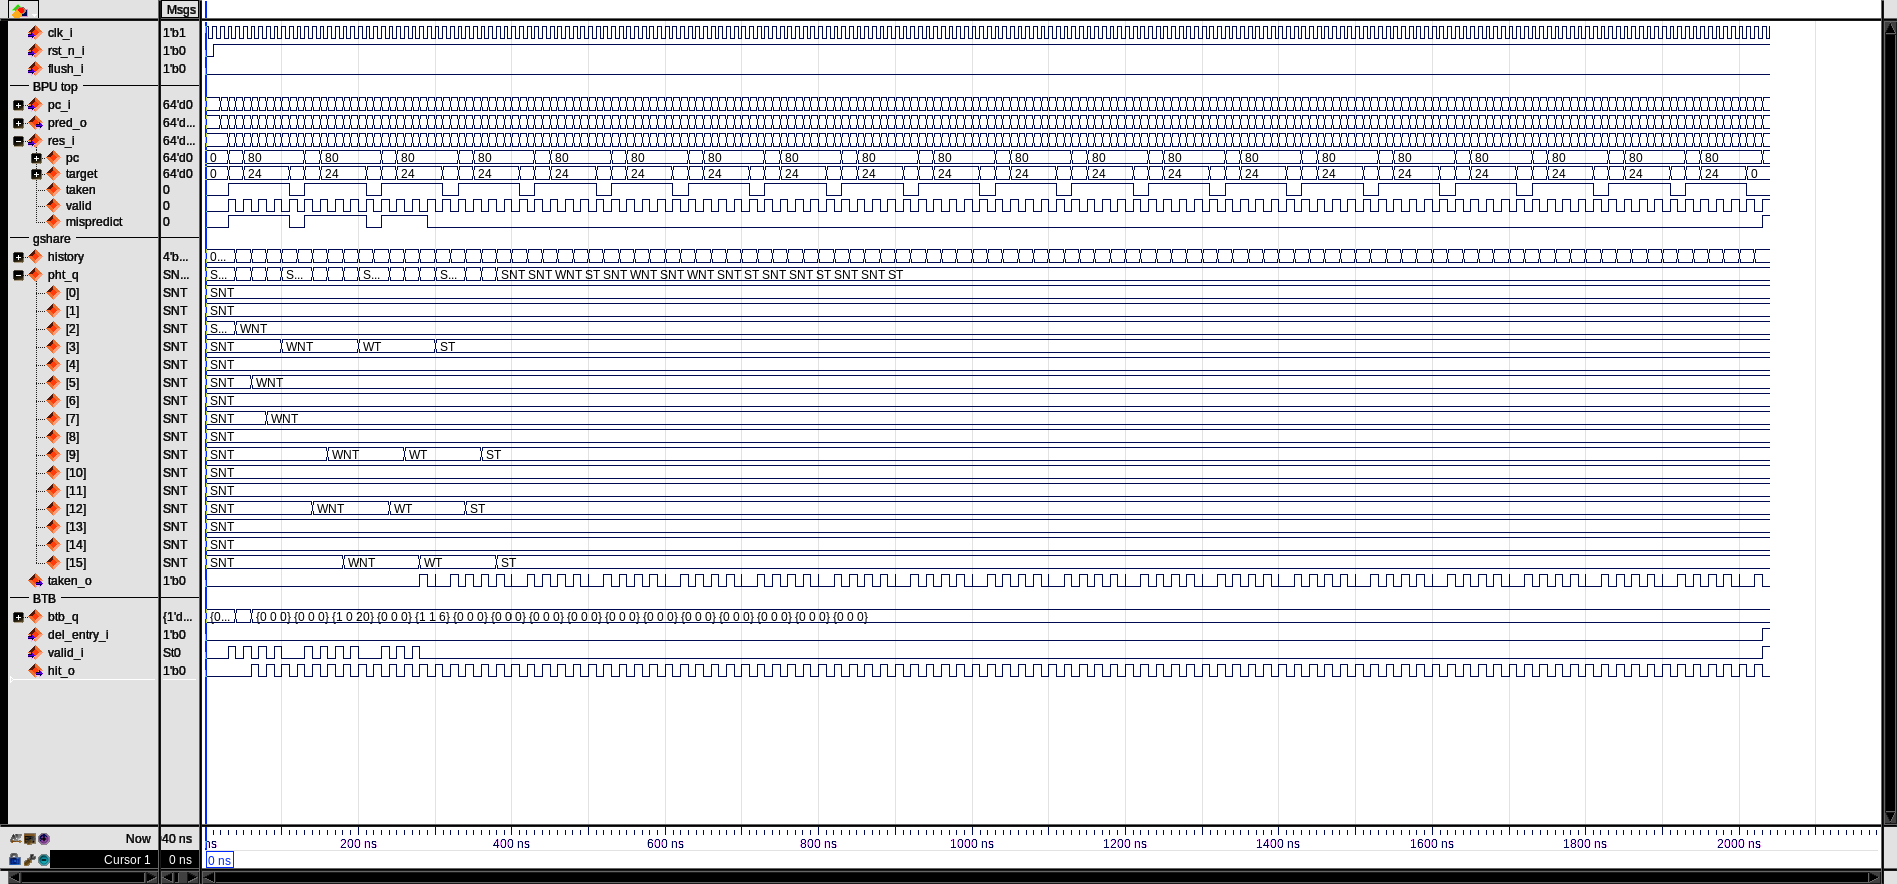
\includegraphics[width=\textheight]{img/bpu_loop02_conv.png}
  \caption{Nested loops simulation}
  \label{fig:bpu_loop02_conv}
\end{sidewaysfigure}
\Cref{fig:bpu_loop02_conv} shows the simulation results for this case, where the address of the condition instruction of the outer loop is 10, the one of the inner loop (i.e. the target of the outer loop) is 80 and the body of the inner loop starts at address 24. 

At the beginning, the gshare continuously mispredicts the outer loop and the first iterations of the inner loop, due to the initialization of the \ac{PHT} as mentioned in the previous case, but then after the warm-up it goes on to predict correctly both loops, until the exit of the outer loop. In particular, the steady state situation is shown in \cref{tab:nested}, where each combination of address and history univocally determines the prediction outcome.
\begin{table}[hbt]
  \centering
  \begin{tabular}{lllll}
    \toprule
    \textbf{Value} & \textbf{Condition} & \textbf{\ac{PC}} & \textbf{History} & \textbf{Prediction} \\ \midrule
    \texttt{j = 0} & \texttt{j < 3}   & 80  & 1101  & Taken     \\ \midrule
    \texttt{j = 1} & \texttt{j < 3}   & 80  & 1011  & Taken     \\ \midrule
    \texttt{j = 2} & \texttt{j < 3}   & 80  & 0111  & Taken     \\ \midrule
    \texttt{j = 3} & \texttt{j < 3}   & 80  & 1111  & Not taken \\ \midrule
    \texttt{i = n} & \texttt{i < 20}  & 10  & 1110  & Taken     \\
    \bottomrule
  \end{tabular}
  \caption{Nested loops steady state predictions}
  \label{tab:nested}
\end{table}

\subsection{Frontend}
The testbench designed for the whole frontend is composed of the following blocks that drive its inputs:
\begin{itemize}
  \item A \emph{\ac{PC} jumper} used to simulate exceptions and branches by modifying the sequential generation of addresses.
  \item A \emph{dummy instruction cache} which responds to memory access requests by simulating both hits and misses, with random delays. The fictional data line it provides always contains the \ac{PC} that generated the request and $N$ instruction fields with the number from 1 to $N$ in order to track the movement of instructions.
  \item A \emph{dummy issue queue} that simply simulates a busy issue queue by introducing random delays on the \texttt{issue\_ready} signal.
\end{itemize}

Using this setup, the frontend was simulated in a number of scenarios corresponding to the different situations analyzed in \cref{sec:frontend_timings}, of which the most significant are described below.

\Cref{fig:fetch01_conv} shows the standard situation where subsequent instructions are selected among the same line, saved in the line register after the first memory access at startup (compare with \cref{fig:fetch01}).

\Cref{fig:fetch02_address_conv,fig:fetch02_miss_conv} show the situation of a cache not ready to receive the address or a cache miss respectively, as in \cref{fig:fetch02}. Note also the current states of the instruction cache interface \acs{FSM} that correspond to the timing diagrams of \cref{fig:cache02,fig:cache03}\footnote{These simulation waveforms show \texttt{WAIT\_ADDR} as the wrong old name for the \texttt{WAIT\_REQ} state.}.

\Cref{fig:fetch07_conv} shows a sequence of cache reads in a pipeline fashion, just as in \cref{fig:fetch07}. Note also how here there is a jump right after the boot address, which is correctly handled by the instruction cache interface.

\Cref{fig:fetch09_conv}, like \cref{fig:fetch09}, show the case when the instruction is selected among the line backup register, due to a jump back and forth to the same cache line.

Finally as an example, \cref{fig:fetch03_conv} shows the situation in which the issue queue is not ready during instruction selection (compare with \cref{fig:fetch03}).

\begin{sidewaysfigure}[p]
  \centering
  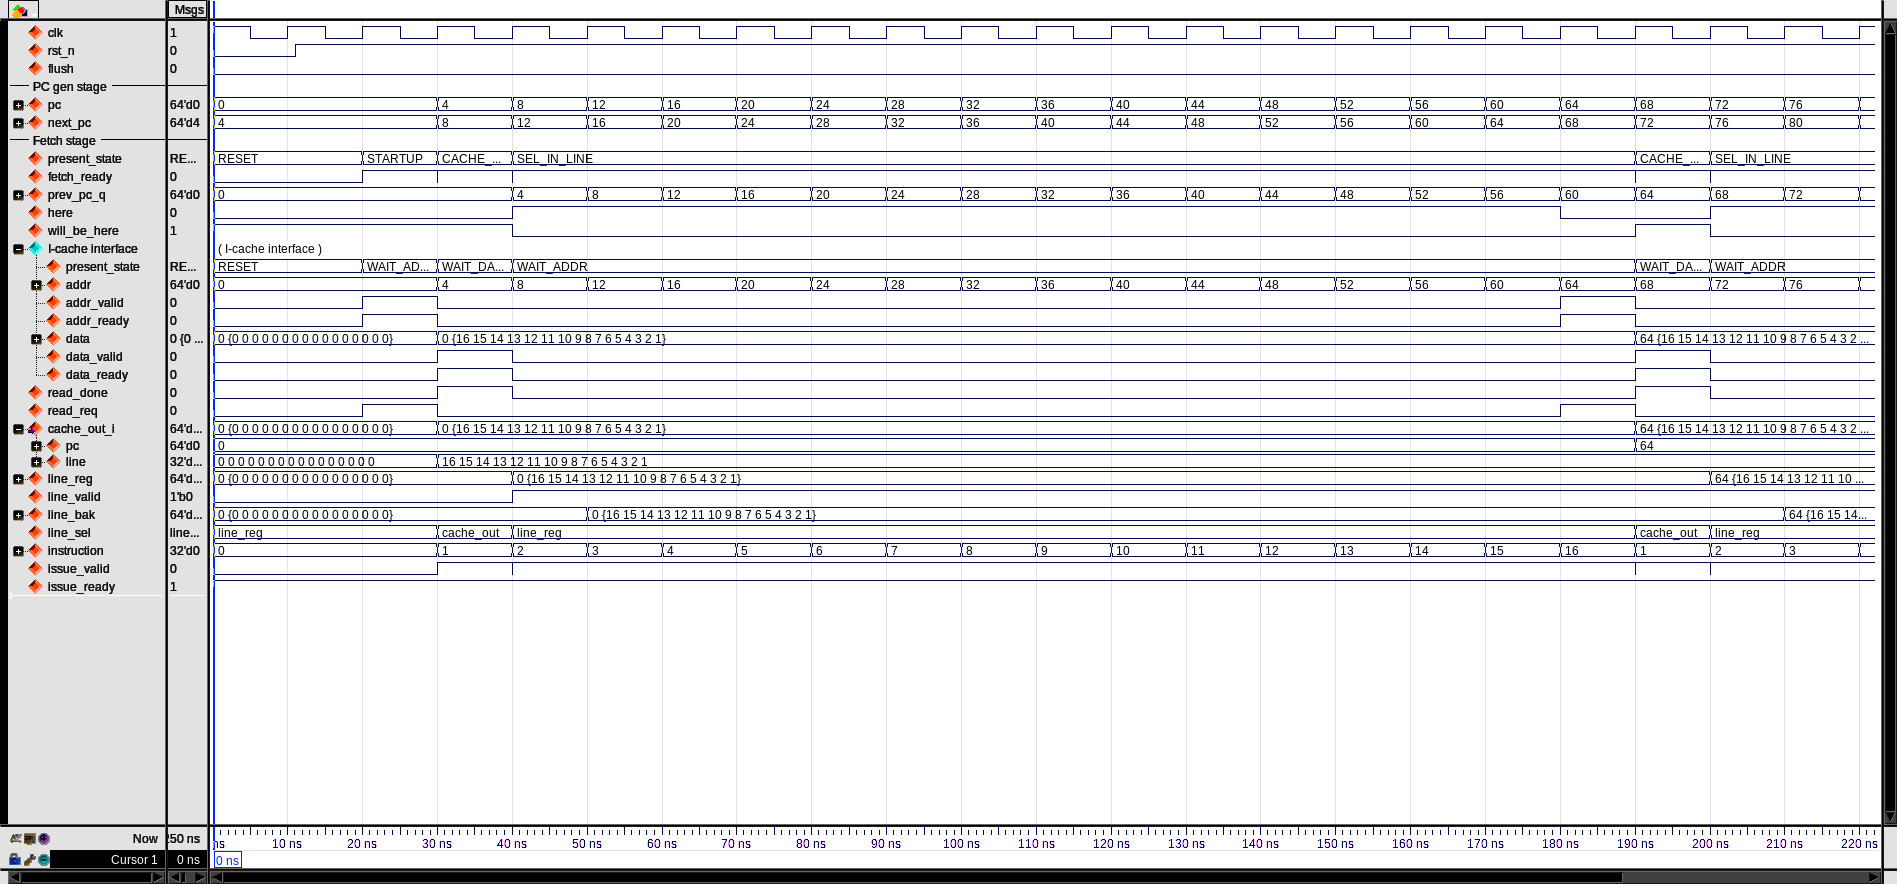
\includegraphics[width=\textheight]{img/fetch01_conv.png}
  \caption{Sequential reads from the same line}
  \label{fig:fetch01_conv}
\end{sidewaysfigure}
\begin{sidewaysfigure}[p]
  \centering
  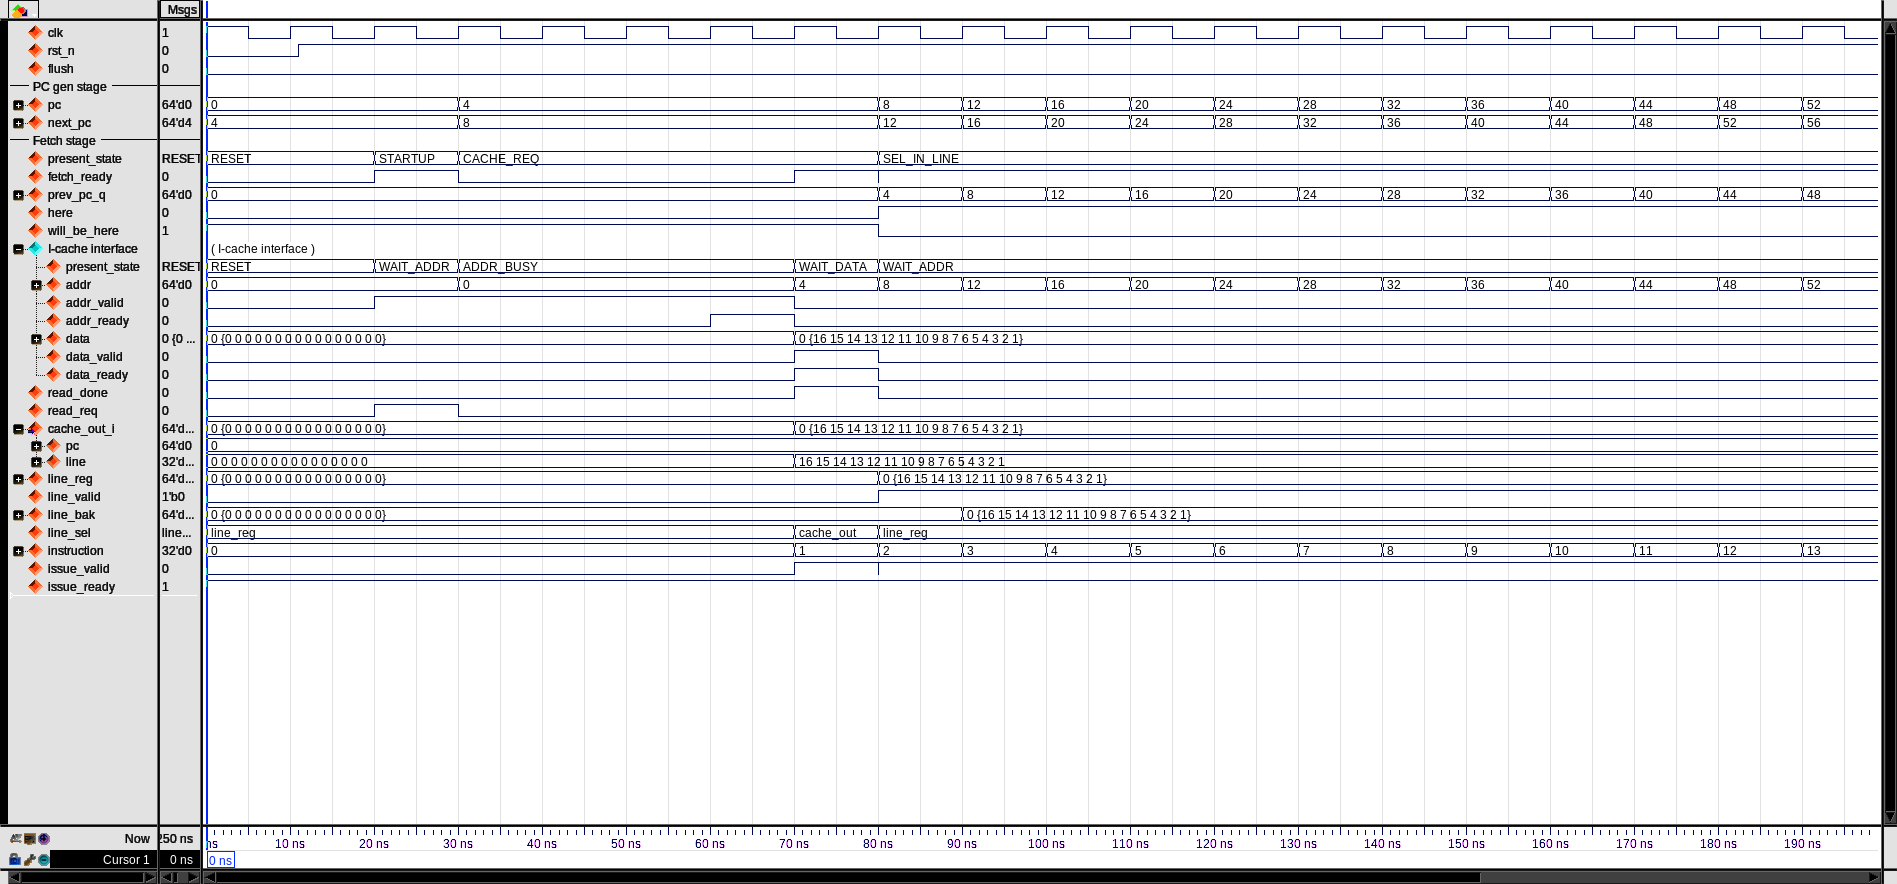
\includegraphics[width=\textheight]{img/fetch02_address_conv.png}
  \caption{Cache not ready on address}
  \label{fig:fetch02_address_conv}
\end{sidewaysfigure}
\begin{sidewaysfigure}[p]
  \centering
  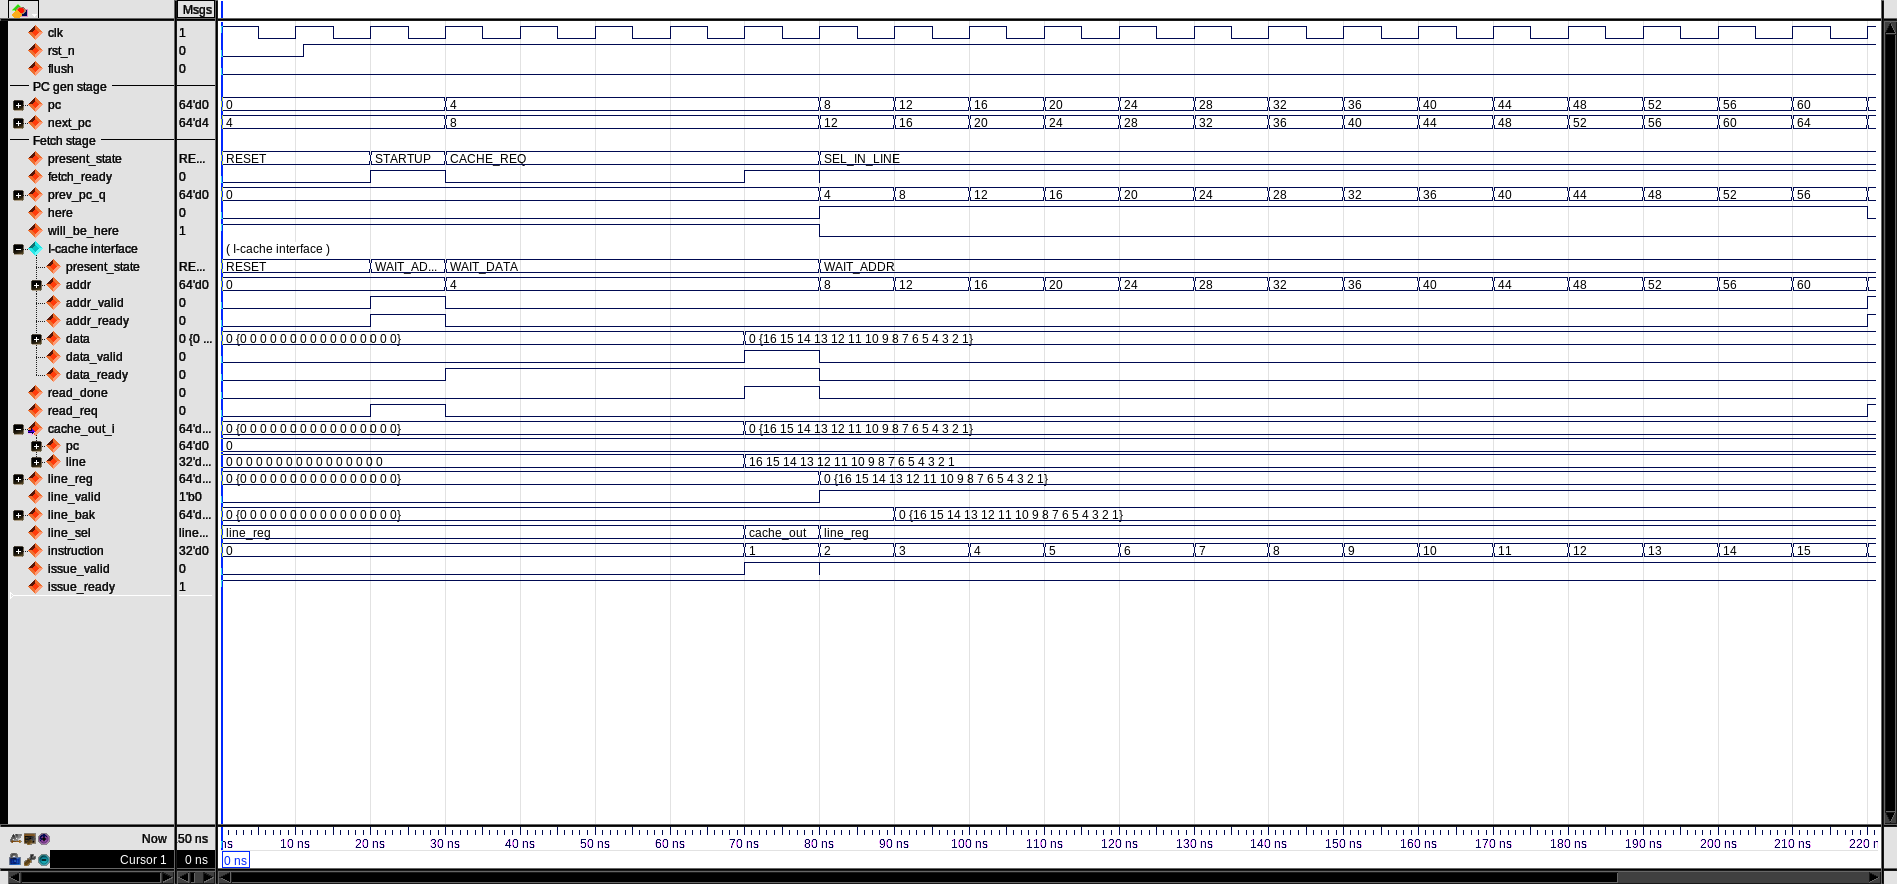
\includegraphics[width=\textheight]{img/fetch02_miss_conv.png}
  \caption{Cache miss}
  \label{fig:fetch02_miss_conv}
\end{sidewaysfigure}
\begin{sidewaysfigure}[p]
  \centering
  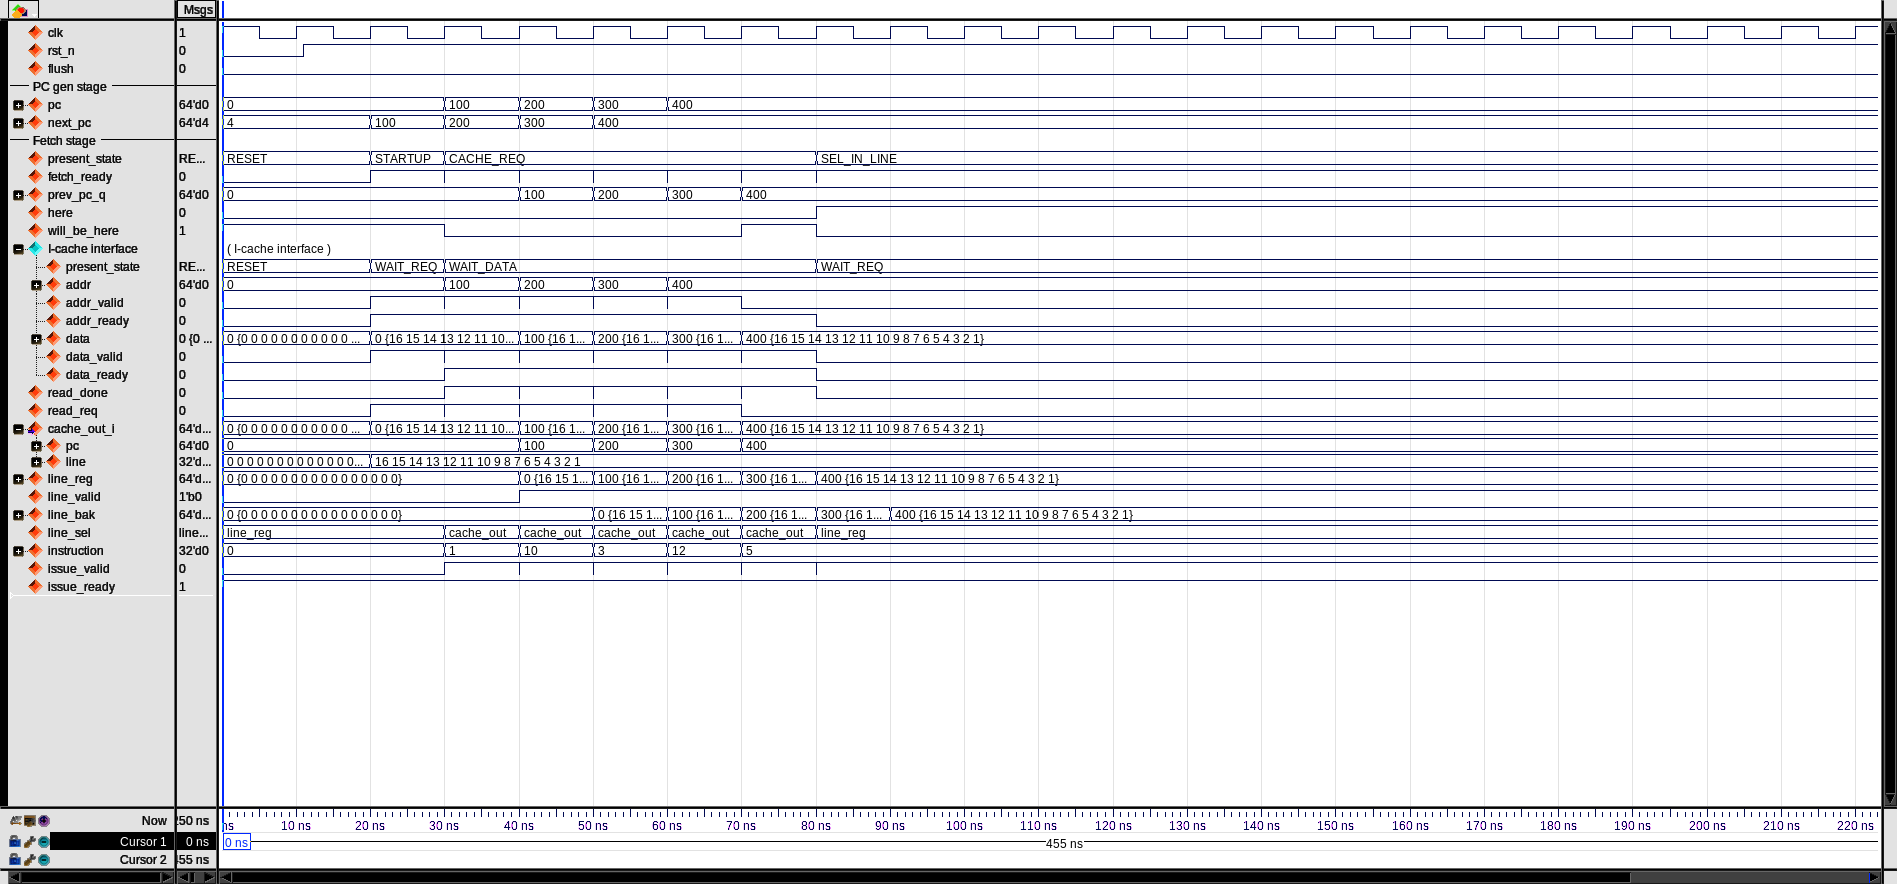
\includegraphics[width=\textheight]{img/fetch07_conv.png}
  \caption{Cache read pipeline}
  \label{fig:fetch07_conv}
\end{sidewaysfigure}
\begin{sidewaysfigure}[p]
  \centering
  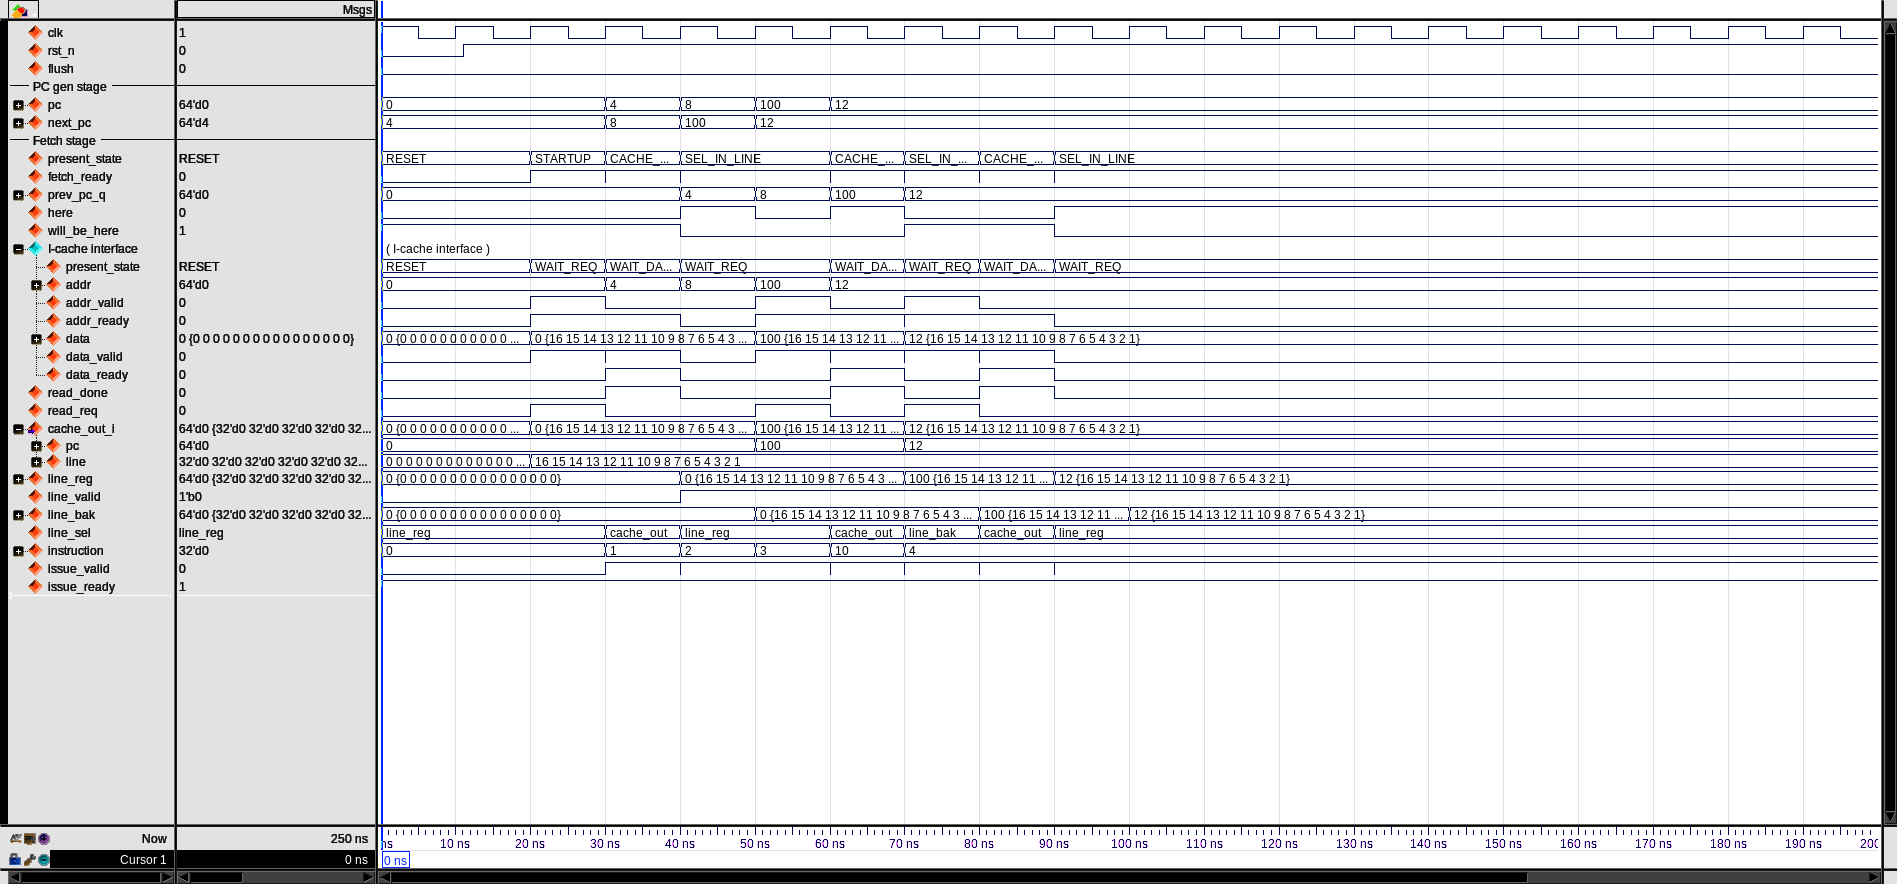
\includegraphics[width=\textheight]{img/fetch09_conv.png}
  \caption{Line backup register selection}
  \label{fig:fetch09_conv}
\end{sidewaysfigure}
\begin{sidewaysfigure}[p]
  \centering
  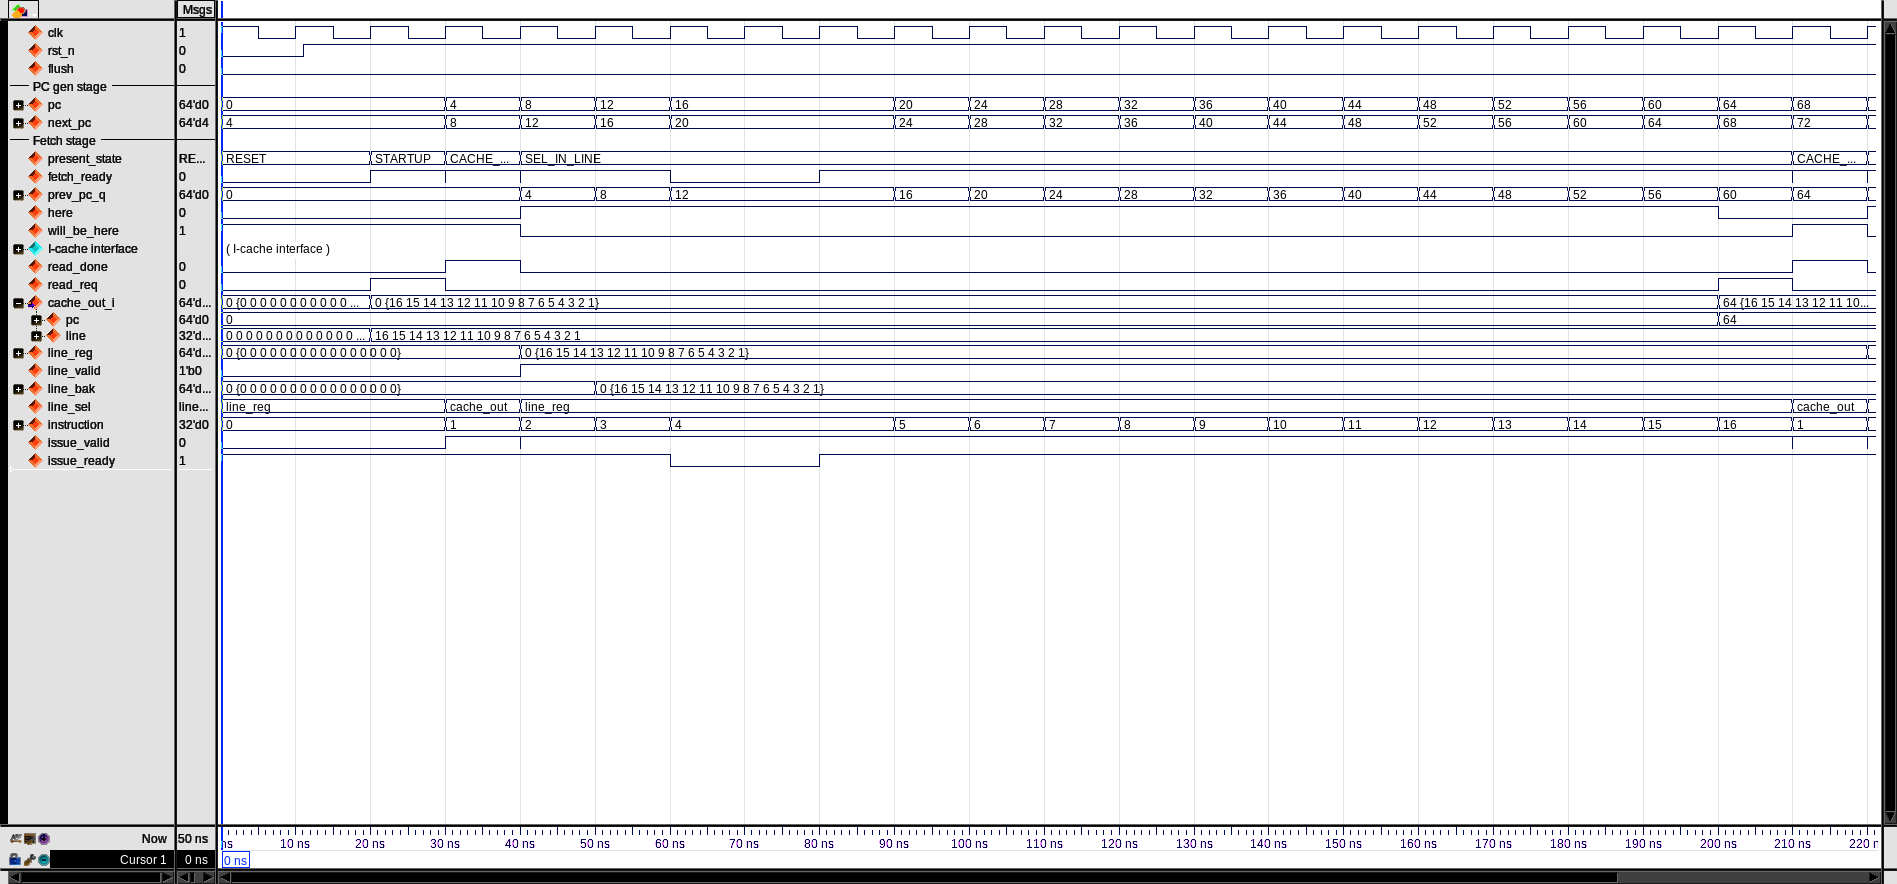
\includegraphics[width=\textheight]{img/fetch03_conv.png}
  \caption{Issue queue busy}
  \label{fig:fetch03_conv}
\end{sidewaysfigure}

\section{\acs{BPU} benchmarking}
As mentioned before, the \ac{BPU} is one of the most configurable units in the design, where a number of parameters and design choices come into play. For this reason a software model of this module written in C has been developed, to allow for fast and simple exploration and benchmarking. The model implements the same functions as the hardware and reads an input text file in the form
\begin{center}
  \texttt{<BRANCH ADDRESS>}  \texttt{<OUTCOME>}
\end{center}
where the address is expressed in hexadecimal base and the outcome as 1 or 0 if the branch is taken or not.

After significant efforts spent to find a way to extract \emph{branch traces} (i.e. the list of branch instructions and their result) from a compiled program, no feasible solution was found and so a decision was made to rely on the trace files provided by a laboratory exercise of the course \emph{Principles in Computer Architecture} held by Prof. Dean Tullsen of the University of California San Diego, available on GitHub\footnote{\url{https://github.com/prodromou87/CSE240A}}. These traces come from a series of benchmarks taken from the SPEC suite, listed in \ref{tab:benchmarks}.
\begin{table}[hbt]
  \centering
  \begin{tabular}{lll}
    \toprule
    \textbf{Name}   & \textbf{Type}    & \textbf{Branches}  \\ \midrule
    \texttt{fp\_1}  & Floating point   & \num{1546797}      \\ \midrule
    \texttt{fp\_2}  & Floating point   & \num{2422049}      \\ \midrule
    \texttt{int\_1} & Integer          & \num{3771697}      \\ \midrule
    \texttt{int\_2} & Integer          & \num{3755315}      \\ \midrule
    \texttt{mm\_1}  & Matrix multiply  & \num{3014850}      \\ \midrule
    \texttt{mm\_2}  & Matrix multiply  & \num{2563897}      \\
    \bottomrule
  \end{tabular}
  \caption{\acs{BPU} benchmarks}
  \label{tab:benchmarks}
\end{table}

In the following sections, a series of tests is described to evaluate performance and other design metrics on the \ac{BPU}.

\subsection{Gshare}\label{sec:gshare_bench}

\subsection{\acs{BTB}}

\section{Synthesis}